\section{Eqiuvalent of linear functions for PARTITION}\label{evalSec:onemax}
The input of this section is more or less equivalent to linear functions. All values except the first follow any distribution whereas the first value is the sum of all other values.
The optimal solution is therefore the 100\dots00 or the 011\dots11 string.
So the input is almost identical to a linear function with positive weights that is maximised/minimised depending on the value of the first bit.\newline
For linear functions the mutation rate of 1/n was proven to be optimal for the (1+1) EA~\cite{witt2013tight}.
This should also hold for this input.
The RLS variants should also perform worse than the standard RLS.\
The higher the value for $\beta$ the better the $pmut_\beta$ mutation should perform.
Flips of the first bits could decrease the runtime, depending on how often they happen.
By doing some testing with various algorithm variants of the RLS and the (1+1) EA it looked like the first bit was only flipped at most once for every input.
There was only one case where it was flipped twice, but it was never flipped more than twice per run.
The average number of flips was also mostly closer to zero than to one.\newline
The experiments where conducted with the variant where the smaller values are all one.
So for every run of each algorithm the input was $[n-1, 1, 1, \dots, 1, 1]$.
An input like this takes less time for every algorithm, but the results are mostly the same.
\subsection{RLS Comparison}
\makebox[\linewidth]{
\begin{tabular}{lp{3cm}p{6cm}p{6cm}}
\begin{tabular}[h]{cccccccc}
algo type&            \RLSN&     \RLSR&     \RLSR&     \RLSN&     \RLSR&     \RLSN&       RLS\\
algo param&             b=2&       s=3&       s=4&       b=3&       s=2&       b=4&         -\\
avg mut/change&       2.000&     1.996&     2.476&     3.000&     1.502&     4.000&     1.000\\
avg mut/step&         2.000&     2.000&     2.500&     3.000&     1.500&     4.000&     1.000\\
\hline
total avg count&     83,118&   104,748&   105,513&   112,223&   114,486&   121,927& 2,443,567\\
avg eval count&      83,118&   104,748&   105,513&   112,223&   114,486&   121,927&    45,834\\
max eval count&     778,110& 1,453,252&   898,974& 1,377,471&   915,268&   816,633&   485,275\\
min eval count&         197&       126&        45&       212&       271&       155&       128\\
\hline
fail ratio&           0.000&     0.000&     0.000&     0.000&     0.000&     0.000&     0.447\\
avg fail dif&             -&         -&         -&         -&         -&         -&         1\\
\end{tabular}
\end{tabular}
}

As expected the standard RLS reaches an optimal solution the fastest.
It also reaches an optimal value for every instance.
The \RLSR[s] variants need more iterations to find an optimal solution.
By looking at the average values more closely it seems like the average number of steps for the \RLSR[s] is roughly $25,000 + 70,000s \pm 5,000$.
The standard RLS is equivalent to \RLSR~or \RLSN~with $k=1$.
So the value of $k=1$ seems to be optimal for the RLS variants.
The \RLSN[b] variants on the other hand do not reach any of the two optimal solutions in any run.
This is most likely caused by their very low possibility of flipping only one bit in a single step.
They would eventually reach the optimal solution as well, but this would take much longer than for the RLS.\
The probability of flipping only one bit in a step is $\mathcal{O}(n^{1-k})$ which results in a single bit flip every $\Omega(n^{k-1})$ steps in expectation.
Because the fitness can only improve for OneMax making steps flipping more bits does not harm the fitness.
The bound for OneMax is $\mathcal{O}(n\log n)$ and with the previous result the expected number of steps is bounded by
$\mathcal{O}(n\cdot\mathcal{O}(n^{k-1})\cdot \log(n\cdot\mathcal{O}(n^{k-1}))) 
=\mathcal{O}(n^{k-1+1}\cdot (k-1+1)\cdot\log(n))
=\mathcal{O}(kn^{k}\cdot\log(n))$
This problem is not equivalent to OneMax, as a flip of the bit with the highest value inverts the fitness function to ZeroMax but the result might still hold as the bound for the standard RLS for this input is the same as for the RLS on OneMax.
There is no statistically significant difference between the \RLSN[b] variants because all variants reached the step limit in each run.
Only the amount of steps was used to for the significance test, so it looks like all variants are the same.
If the test was executed with the differences to the optimum there would be a statistically significant difference between each algorithm.
\subsection{(1+1) EA Comparison}
\makebox[\linewidth]{
\begin{tabular}{lp{3cm}p{6cm}p{6cm}}
\begin{tabular}[h]{ccccccccc}
algo type&          (1+1) EA&   (1+1) EA&   (1+1) EA&   (1+1) EA&      (1+1) EA&   (1+1) EA&   (1+1) EA&   (1+1) EA\\
algo param&           3/n&     4/n&     2/n&     5/n&       -&    10/n&    50/n&   100/n\\
avg mut/change&     3.101&   3.968&   2.343&   4.859&   1.698&   9.732&  49.544&  99.494\\
avg mut/step&       2.999&   4.003&   2.002&   4.999&   1.001&   9.998&  49.998&  99.997\\
\hline
total avg count&      646&     701&     706&     857&   1,123&   1,508&   8,175&  15,485\\
avg eval count&       646&     701&     706&     857&   1,123&   1,508&   8,175&  15,485\\
max eval count&     5,346&   5,692&   3,415&   5,572&   7,001&  12,112&  52,831& 145,269\\
min eval count&        23&       4&      30&       9&      23&      14&      27&      69\\
\hline
fails&                  0&       0&       0&       0&       0&       0&       0&       0\\
fail ratio&         0.000&   0.000&   0.000&   0.000&   0.000&   0.000&   0.000&   0.000\\
avg fail dif&           -&       -&       -&       -&       -&       -&       -&       -\\
\end{tabular}
\end{tabular}
}

For this input the same as for OneMax holds. 
The static mutation rate $p_m=1/n$ is the optimal value and the performance of the (1+1) EA decreases with rising mutation rate.
Only for $p_m\le2/n$ the (1+1) EA managed to find one of the two optimal solutions in $10 \cdot n\ln(n)$ steps every time.
With mutation rate $p_m=4/n$ the (1+1) EA only managed to find the optimal solution in about 50 \% of the inputs.
The remaining mutation rates did not manage to find an optimal solution in any of the runs.
Another interesting fact is the average number of bits flipped in a successful step.
For the other inputs the overall average number of bits flipped in any step was mostly the same as for the average value of the successful steps. Here this is not the case.
All mutation rates flipped fewer bits in the successful steps than in the average step.
The only exception is the standard mutation rate which is caused by the steps where the algorithm would flip no bit.
Those steps decrease the number of the average case but not of the successful case as those steps were skipped.
The p-value between $5/n$ and $10/n$ is 1.0 for the same reason as for the \RLSN[b] variants.
\subsection{pmut Comparison}
For $pmut$ only 1798/10000 repetitions were executed as there was a clear tendency which of the algorithms performs better.

\makebox[\linewidth]{
\scriptsize
\begin{tabular}{lp{3cm}p{6cm}p{6cm}}
\begin{tabular}[h]{m{2.5cm}m{0,40cm}m{0,40cm}m{0,40cm}m{0,40cm}m{0,40cm}m{0,40cm}m{0,40cm}m{0,40cm}m{0,40cm}m{0,40cm}m{0,40cm}m{0,40cm}m{0,40cm}m{0,40cm}m{0,40cm}m{0,40cm}m{0,40cm}m{0,40cm}}
\multicolumn{1}{c}{algo type}&\multicolumn{2}{c}{            pmut}&\multicolumn{2}{c}{     pmut}&\multicolumn{2}{c}{     pmut}&\multicolumn{2}{c}{     pmut}&\multicolumn{2}{c}{     pmut}&\multicolumn{2}{c}{     pmut}&\multicolumn{2}{c}{     pmut}&\multicolumn{2}{c}{     pmut}&\multicolumn{2}{c}{     pmut}\\
\multicolumn{1}{c}{algo param}&\multicolumn{2}{c}{           3.25}&\multicolumn{2}{c}{     3.00}&\multicolumn{2}{c}{     2.75}&\multicolumn{2}{c}{     2.50}&\multicolumn{2}{c}{     2.25}&\multicolumn{2}{c}{     2.00}&\multicolumn{2}{c}{     1.75}&\multicolumn{2}{c}{     1.50}&\multicolumn{2}{c}{     1.25}\\
\multicolumn{1}{c}{avg mut/change}&\multicolumn{2}{c}{      1.583}&\multicolumn{2}{c}{    1.737}&\multicolumn{2}{c}{    2.002}&\multicolumn{2}{c}{    2.423}&\multicolumn{2}{c}{    3.303}&\multicolumn{2}{c}{    5.830}&\multicolumn{2}{c}{   12.519}&\multicolumn{2}{c}{   30.910}&\multicolumn{2}{c}{   73.182}\\
\multicolumn{1}{c}{avg mut/step}&\multicolumn{2}{c}{        1.729}&\multicolumn{2}{c}{    1.934}&\multicolumn{2}{c}{    2.274}&\multicolumn{2}{c}{    2.895}&\multicolumn{2}{c}{    4.360}&\multicolumn{2}{c}{    8.452}&\multicolumn{2}{c}{   22.278}&\multicolumn{2}{c}{   70.532}&\multicolumn{2}{c}{  224.421}\\
\hline
\multicolumn{1}{c}{avg eval count}&\multicolumn{2}{c}{        540}&\multicolumn{2}{c}{      569}&\multicolumn{2}{c}{      594}&\multicolumn{2}{c}{      641}&\multicolumn{2}{c}{      712}&\multicolumn{2}{c}{      808}&\multicolumn{2}{c}{      967}&\multicolumn{2}{c}{    1,285}&\multicolumn{2}{c}{    2,081}\\
\multicolumn{1}{c}{max eval count}&\multicolumn{2}{c}{      3,110}&\multicolumn{2}{c}{    2,891}&\multicolumn{2}{c}{    3,504}&\multicolumn{2}{c}{    3,896}&\multicolumn{2}{c}{    5,152}&\multicolumn{2}{c}{    4,274}&\multicolumn{2}{c}{    5,610}&\multicolumn{2}{c}{    6,190}&\multicolumn{2}{c}{   14,984}\\
\multicolumn{1}{c}{min eval count}&\multicolumn{2}{c}{         22}&\multicolumn{2}{c}{        9}&\multicolumn{2}{c}{       36}&\multicolumn{2}{c}{       25}&\multicolumn{2}{c}{       28}&\multicolumn{2}{c}{       27}&\multicolumn{2}{c}{       27}&\multicolumn{2}{c}{       13}&\multicolumn{2}{c}{       33}\\
\hline
\multicolumn{1}{c}{fail ratio}&\multicolumn{2}{c}{          0.000}&\multicolumn{2}{c}{    0.000}&\multicolumn{2}{c}{    0.000}&\multicolumn{2}{c}{    0.000}&\multicolumn{2}{c}{    0.000}&\multicolumn{2}{c}{    0.000}&\multicolumn{2}{c}{    0.000}&\multicolumn{2}{c}{    0.000}&\multicolumn{2}{c}{    0.000}\\
\hline
\multicolumn{1}{c}{p-value}&&\multicolumn{2}{c}{0.0000}&\multicolumn{2}{c}{0.0000}&\multicolumn{2}{c}{0.0000}&\multicolumn{2}{c}{0.0000}&\multicolumn{2}{c}{0.0000}&\multicolumn{2}{c}{0.0000}&\multicolumn{2}{c}{0.0000}&\multicolumn{2}{c}{0.0000}\\
&&&&&&&&&&&&&&&&&&\end{tabular}
\end{tabular}
}

The results for the $pmut$ operator are pretty similar to the results for the (1+1) EA and the RLS.\
The parameter $\beta=3.25$ which flips the least bits on average finds the solution the fastest.
Decreasing value for $\beta$ lead to more time needed for finding one of the two optima.
All variants find an optimum in every run except for $\beta=1.25$ which has a much higher value for the number of flipped bits per steps.
The average number of bits flipped in a successful mutation is much lower than for the other inputs especially for the lower values for $\beta$.
For the binomial and geometric input the successful average was around 100 for $\beta=1.25$ but for the OneMax equivalent it was only at 5.

\subsection{Comparison of the best variants}
For this comparison neither of the algorithms failed to find one of the two optimal solutions.
The following table lists the amount of iterations the algorithms needed to find an optimal solution.

\begin{tabular}[h]{ccccccccc}
avg&20&50&100&500&1000&5000&10000&50000\\\hline
RLS&32&79&153&579&950&1859&1922&1797\\
\RLSR[2]&391&2124&5005&4218&3530&2362&2160&2229\\
(1+1) EA (1$/n$)&22471&18343&12834&8342&6511&3815&3458&3371\\
(1+1) EA (2$/n$)&16360&9243&6452&4503&4020&3171&3141&3133\\
pmut (3.25)&23440&15929&9658&5644&4406&2434&2162&2172\\
pmut (3.0)&21901&14696&9186&5222&4150&2510&2208&2213\\
\end{tabular}


The results for this experiment are as expected.
The RLS performs better than the (1+1) EA because it does only single bit flips.
The $pmut_{3.25}$ performs better than the standard (1+1) EA although flipping more bits on average.
This is most likely cause by the few steps where $pmut$ flips many bits which increase the average.
But $pmut$ most likely chooses to flip only one bit more often as the (1+1) EA.\
In a previous chapter the $\mathcal{O}(n\log n)$ bound was proven for the (1+1) EA and the RLS (Theorem~\ref{theo:OneMaxResult}).
This seems to hold in practice at least for the easiest version of this input where the small values are one (see Figure~\ref{fig:onemaxNlogNBound}).
The scale of this figure is $n\ln n$ which means that a value of 2 on the $y$-axis means the algorithm needs $2n\ln n$ steps on average to reach the optimal solution.
The standard (1+1) EA performs a bit worse than the other three algorithms and approaches $en\ln n$ instead of staying close to $n\ln n$.

\begin{figure}[h]
      \centering
      \begin{minipage}[b]{0.45\textwidth}
            \caption{Runtime for the OneMax equivalent with a $n\ln(n)$ scale}
            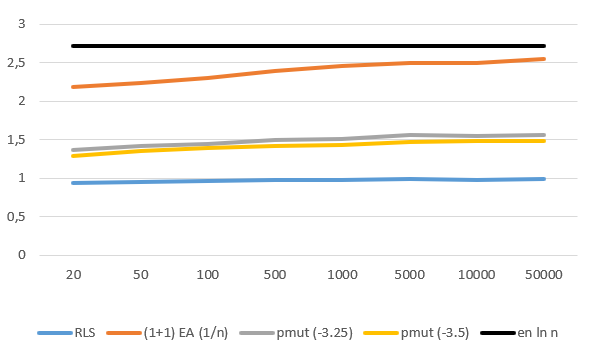
\includegraphics[width=\textwidth]{figures/images/oneMaxMultipleN.png}\label{fig:onemaxNlogNBound}
      \end{minipage}
      \hspace{0.75cm}
      \begin{minipage}[b]{0.45\textwidth}
            \caption{Runtime for the OneMax equivalent with uniform distribution on a $n\ln n$ scale}
            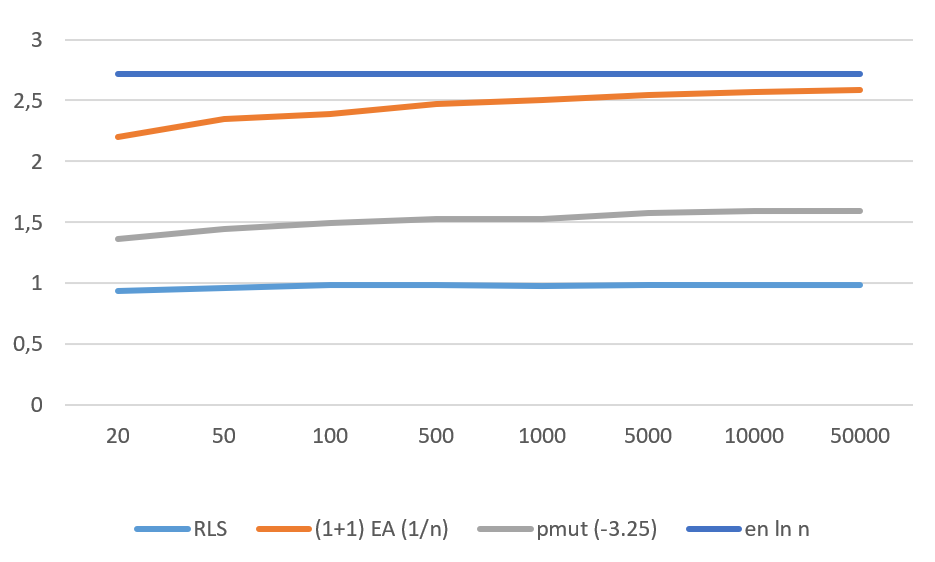
\includegraphics[width=\textwidth]{figures/images/oneMaxUniformMultipleN.png}\label{fig:onemaxUniformNlogNBound}
      \end{minipage}
\end{figure}

Another variant of this input are uniform distributed inputs for example.
The small values in this case are chosen from \textasciitilde$U(1,49999)$ and the first value again is the sum of all other values.
This input is harder because switching multiple small values for a big value decreases the fitness but increases the Hamming distance to the optimum.
Looking at Figure~\ref{fig:onemaxUniformNlogNBound} the equivalent to uniform distributed linear functions looks not much harder compared to the variant where all values are one.
The graphs are almost identical.
It was clear for the RLS because the RLS can't switch elements which leads to the exact same behaviour.
But even the other algorithms that are able to switch seem to not harm the hamming distance drastically by switching elements.

\begin{figure}[h]
      \centering
            \caption{Runtime of the \RLSR~variants for the OneMax equivalent with uniform distribution on a $n\ln n$ scale}
            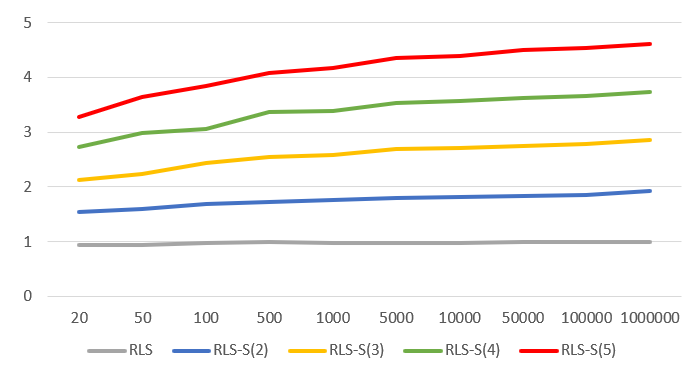
\includegraphics[width=0.5\textwidth]{figures/images/oneMaxUniformMultipleN_RLSRCompare.png}\label{fig:onemaxniformNlogNBoundRLSR}
\end{figure}

Figure~\ref{fig:onemaxniformNlogNBoundRLSR} shows the average number of steps needed by the \RLSR~for the equivalent to linear functions with uniform distribution.
Lemma~\ref{lemma:RLSRoneMaxInput} proved the \RLSR~needs time $4k+\frac{1+o(1)}{1-o(1)}\cdot kn\ln n$ but the actual expected running time seems to be lower.
All \RLSR[k]~variants in the figure approach the value of $kn\ln n$ from below and for at least $n\le50,000$ do not need more time than $kn\ln n$.
The \RLSN[k]~variants on the other hand have a significantly worse performance.
Their average runtime is shown in Figure~\ref{fig:onemaxniformNlogNBoundRLSB} with a logarithmic $y$-axis.
A value of 2 on the $y$-axis here means that the algorithm needed $n^2$ steps on average to find an optimal solution.
All \RLSN[k] variants needs at least almost $n^2$ steps on average, but all variants seem to approach $n^k$ from below (see Lemma~\ref{lemma:RLSNBad}).
The actual runtime is below $n^k$ for greater values of $k$ and smaller input sizes which is likely a consequence of the constants.
For small input sizes $k!$ has a much higher impact but the more $n$ grows the less noticeable the constant becomes.
Figure~\ref{fig:onemaxniformNlogNBoundRLSBWeirdScale} shows their runtime on a different scale.
A value of 2 on the $y$-axis here means that the algorithm needed $n^2/k!$ steps on average to find an optimal solution where $k$ is dependent on the algorithm.
So all \RLSN[k] variants needed about $n^k/k!$ steps on average to find an optimal solution for any input size.
This is exactly the lower bound proven in Lemma~\ref{lemma:RLSNBad}.
% With the less strict lower bound of $\frac{n^k}{k!}$ proven in the Lemma for small values of $n$ the constant $k!$ matters.
% This is why the higher the value of $k$ the less clear the asymptotic runtime appears.
% Testing higher values for $k=4$ should reveal a better view on the asymptotic runtime but if the asymptotic runtime is actually close to $n^4$ then it would take $1000^4=10^{12}$ steps for $n=1000$.
% With a runtime that high it was out of this thesis time budget to test multiple runs of the \RLSN[4] with higher input sizes.

\begin{figure}[h]
      \centering
      \begin{minipage}[b]{0.45\textwidth}
            \caption{Runtime of the \RLSN~variants for the OneMax equivalent with uniform distribution on a $n^y$ scale}
            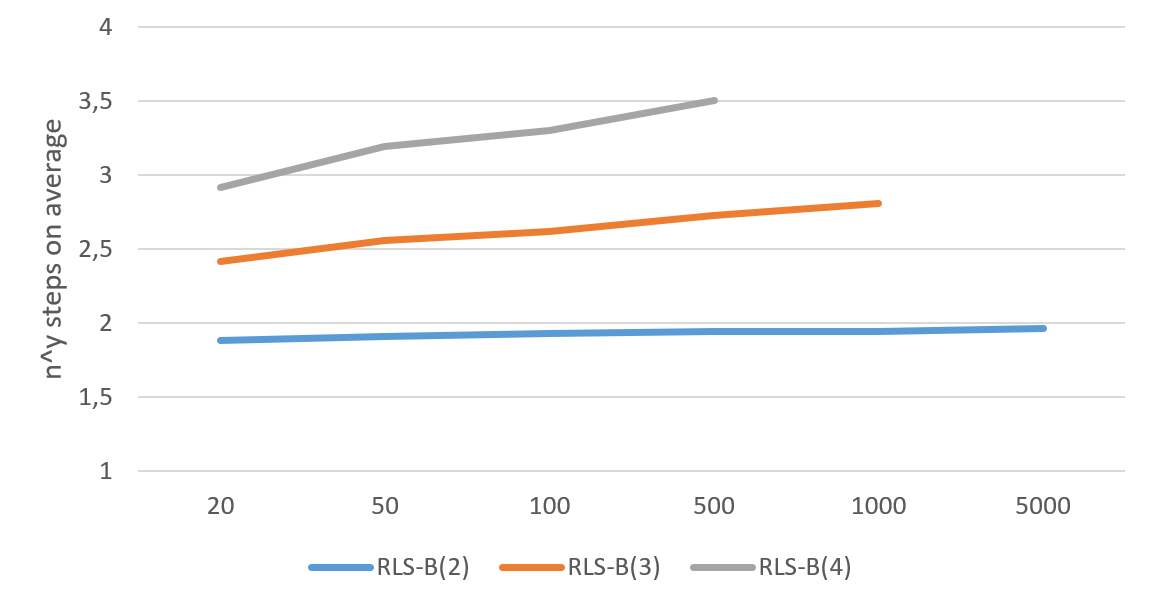
\includegraphics[width=\textwidth]{figures/images/oneMaxUniformMultipleN_RLSBCompare.png}\label{fig:onemaxniformNlogNBoundRLSB}
      \end{minipage}
      \hspace{0.75cm}
      \begin{minipage}[b]{0.45\textwidth}
            \caption{Runtime of the \RLSN~variants for the OneMax equivalent with uniform distribution on a $n^y/k!$ scale}
            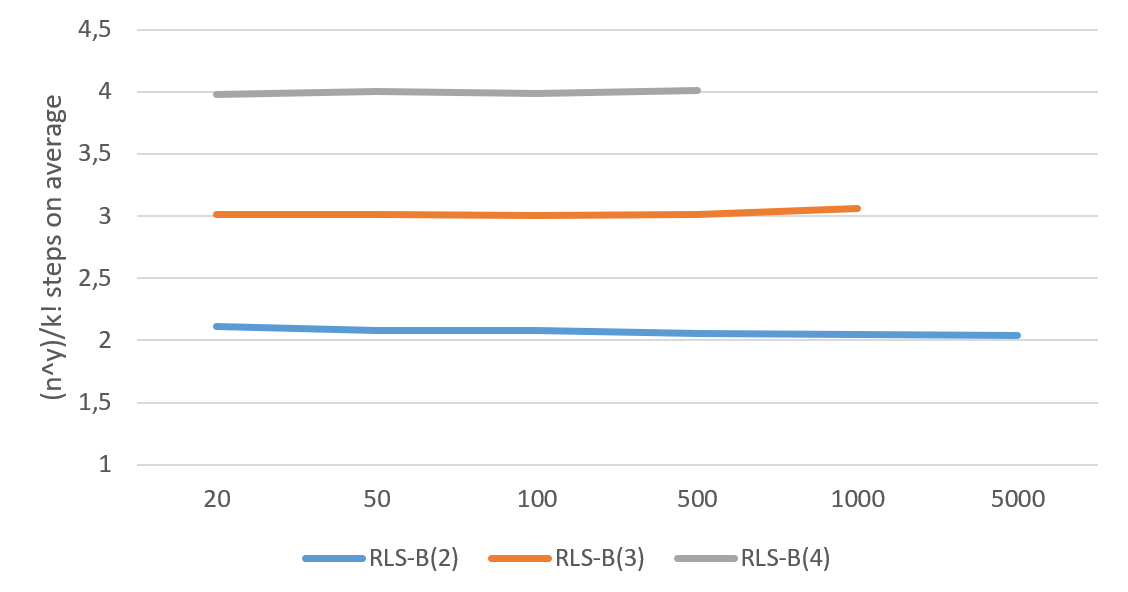
\includegraphics[width=\textwidth]{figures/images/oneMaxUniformMultipleN_RLSBCompareScaleWithConstant.png}\label{fig:onemaxniformNlogNBoundRLSBWeirdScale}
      \end{minipage}
\end{figure}
The bound proven for the (1+1) EA with mutation rate $c/n$ was \(4+\frac{3+o(1)}{1-o(1)}\cdot \frac{e^c}{c}n\ln n\) (Theorem~\ref{theo:OneMaxResult}) but looking at Figure~\ref{fig:onemaxuniformEA} the actual bound seems more like \(\frac{e^c}{c}n\ln n\).
For $pmut$ there was no proof in this thesis but the bigger values of $pmut$ also seem to take time $\Theta(n\ln n)$ (Figure~\ref{fig:onemaxniformPmut}).

\begin{figure}[h]
      \centering
      \begin{minipage}[b]{0.45\textwidth}
            \caption{Runtime of the (1+1) EA for the OneMax equivalent with uniform distribution on a $n\ln n$ scale}
            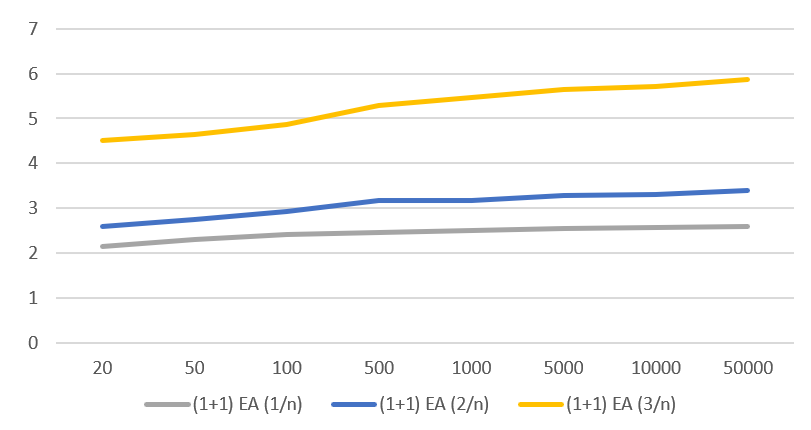
\includegraphics[width=\textwidth]{figures/images/oneMaxUniformMultipleN_EACompareNlnn.png}\label{fig:onemaxuniformEA}
      \end{minipage}
      \hspace{0.75cm}
      \begin{minipage}[b]{0.45\textwidth}
            \caption{Runtime of $pmut$ for the OneMax equivalent with uniform distribution on a $n\ln n$ scale}
            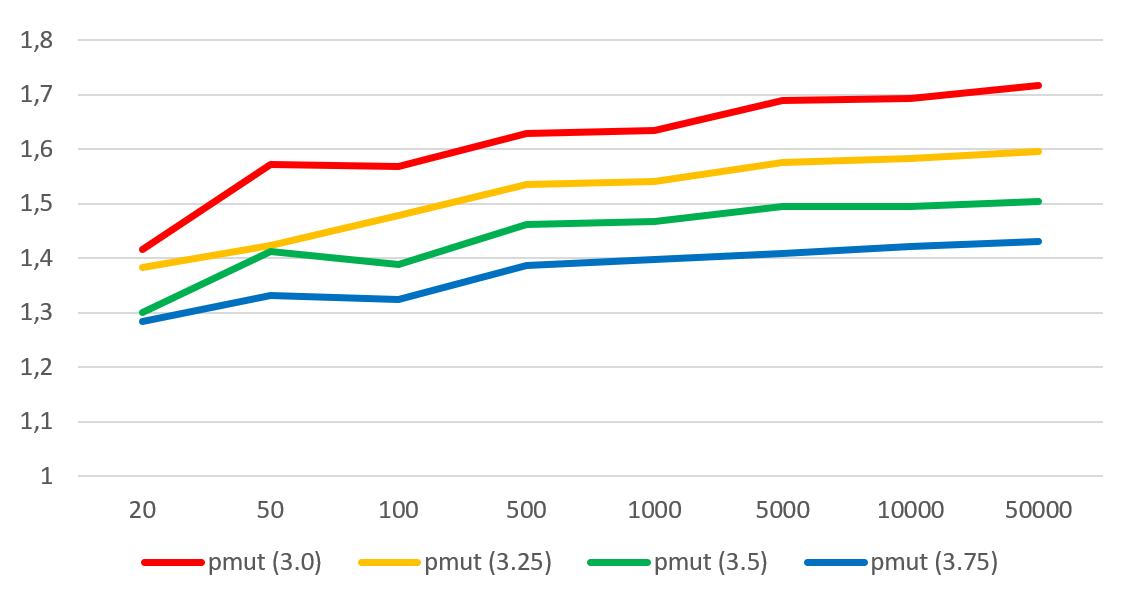
\includegraphics[width=\textwidth]{figures/images/oneMaxUniformMultipleN_pmutCompare.png}\label{fig:onemaxniformPmut}
      \end{minipage}
\end{figure}